\documentclass[11pt,letterpaper]{article}


\usepackage[utf8]{inputenc}
\usepackage[spanish]{babel}
\usepackage{float}
\usepackage{xcolor}
\usepackage{verbatim}
\usepackage{mwe}
\usepackage{charter}
\usepackage{afterpage}
\usepackage{amsmath}
\usepackage{appendix}
\usepackage{ragged2e}
\usepackage{array}
\usepackage{etoolbox}
\usepackage{fancyhdr}
\usepackage{booktabs}
\usepackage{arydshln}
\usepackage[justification=justified,singlelinecheck=false,labelfont=bf,format=plain]{caption}
\usepackage[justification=justified,singlelinecheck=false,labelfont=bf,format=plain]{subcaption}
\usepackage{enumitem}
\usepackage[bottom=2.5cm,top=2.0cm,left=2.0cm,right=2.0cm]{geometry}
\usepackage{graphicx}
\usepackage{indentfirst}
\usepackage{mathtools}
\usepackage{multirow}
\usepackage{pdfpages}

\usepackage{subfiles}
\usepackage[compact]{titlesec}
\usepackage{blindtext}
\usepackage{stfloats}
\usepackage{lipsum} 
\usepackage{import}
\usepackage{pdfpages}
\usepackage{transparent}
\usepackage{xcolor}
\usepackage[colorlinks=true,linkcolor=blue]{hyperref}


\newcommand{\incfig}[2][1]{%
	    \def\svgwidth{#1\columnwidth}
	        \import{../img/}{#2.pdf_tex}
	}

	\pdfsuppresswarningpagegroup=1
\renewcommand{\familydefault}{\rmdefault}
\newcommand\blankpage{
    \null
    \thispagestyle{empty}
    \addtocounter{page}{0}
    \newpage}

\newcolumntype{L}[1]{>{\raggedright\let\newline\\arraybackslash\hspace{0pt}}m{#1}}
\newcolumntype{C}[1]{>{\centering\let\newline\\arraybackslash\hspace{0pt}}m{#1}}
\newcolumntype{R}[1]{>{\raggedleft\let\newline\\arraybackslash\hspace{0pt}}m{#1}}

    \setlist[itemize,1]{label=$\bullet$}
    \setlist[itemize,2]{label=$\circ$}
    \setlist[itemize,3]{label=$-$}
    \setlist{nosep}

\setlength{\columnsep}{30pt}

\titlelabel{\thetitle.\quad}

\pagestyle{fancy}
\fancyhf{}
      
\fancyfoot{}
\fancyfoot[C]{\thepage} % page
\renewcommand{\headrulewidth}{0mm} % headrule width
\renewcommand{\footrulewidth}{0mm} % footrule width

\makeatletter
\patchcmd{\headrule}{\hrule}{\color{black}\hrule}{}{} % headrule
\patchcmd{\footrule}{\hrule}{\color{black}\hrule}{}{} % footrule
\makeatother

\definecolor{blueM}{cmyk}{1.0,0.49,0.0,0.47}

%%%%%%%%%%%%%%%%%%%%%%%%%%%%%%%%%%%%%%%%%%%%%%%%%%%%%%%%%%%%%%%%%%%%%%%%%%%%%%%%%%%%%%%%%%%%%%%%%%%%%%%%%%%%%%%%%%%%%%%%%%%%%%%%%%%%%%%%%%%%%%%%%%%%%%%%%%%%%%%%%%%%%%%%%%%%%%%%%%%%%%%%%%%%%%%%%%%%%%%%%%%%%%
%%%%%%%%%%%%%%%%%%%%%%%%%%%%%%%%%%%%%%%%%%%%%%%%%%%%%%%%%%%%%%%%%%%%%%%%%%%%%%%%%%%%%%%%%%%%%%%%%%%%%%%
\title{RLC salida en C}    
\author{Álvaro Martín Romero}
\begin{document}
\maketitle
\tableofcontents
\section{Ejercicio 1}%
\label{sec:Muestra del circuito}
\subsection{Valor de la tensión de salida para la frecuencia de corte}
La tensión de salida para el circuito dado en salida de $R$ es:
\[
V_s=\frac{\frac{V_e}{Cs}}{Ls+\frac{1}{Cs}+R}
.\] 
Hallamos la función de transferencia de este circuito utilizando su definición:
\[
    G\left( s \right) =\frac{V_s}{V_e} \implies G\left( s \right) =\frac{1}{\left( LCs^2+ RCs + 1 \right) }
.\] 
Haciendo $w_n=\frac{1}{\sqrt{LC} }$ y $RC=\frac{2\zeta}{w_n}$ con el cambio $s=j\omega$ el módulo de la función de transferencia es:
 \[
     G\left( j\omega \right) =\frac{1}{\sqrt{\left( 1-\frac{\omega^2}{\omega_n^2} \right)^2+ \left( \frac{2\zeta \omega }{\omega_n} \right)^2  } } \mid V_e\left( j\omega \right)  \mid   
.\] 
Por tanto, si multiplicamos el módulo de la función de transferencia por la tensión de entrada y sustituimos los datos que nos da el problema $[R=220 \Omega ; L=10 mH; C=10nF; V_e =20Vpp=10 V]$:

\[
	\omega_{n}=\frac{1}{\sqrt{LC} }\implies f_n=\frac{1}{2\pi}\cdot \frac{1}{LC}=[L=10 mH; C= 10 nF]=15915.494 Hz 
.\] 
y 
 \[
	 \zeta=\frac{R}{2L}\sqrt{LC} =[R= 220 \Omega] =0.11
.\] 

Para $\omega=\omega_n= 15915.494Hz$ la tensión de salida calculada de forma teórica es:
\begin{equation}
	\boxed{ \mid V_s \mid = 4.545 \cdot V_e= 45.45 V}
\end{equation}

\subsection{Cálculo del ángulo de desfase}
El ángulo de desfase para el circuito RLC con salida en L se define como:
\begin{equation}
    \varphi= - \arctan\left[ \frac{\frac{2\zeta \omega}{\omega_n}}{\left( 1-\frac{\omega^2}{\omega_n^2} \right) } \right] 
    \label{desfase}
\end{equation}
Donde para la frecuencia de corte: $\frac{\omega}{\omega_n}=1$, por tanto:

\begin{equation}
	\boxed{\varphi=-90^o}
\end{equation}

\subsection{Tensión de salida una década por arriba y por debajo}
\begin{itemize}
	\item Para una década por encima:\\
\\
Esto es: 
\[
\frac{\omega}{\omega_n}=10
.\] 
Sustituyendo ese valor en la función de transferencia y despejando, nos queda que la tensión de salida es:
\begin{equation}
	\boxed{V_s=0.10 V}
\end{equation}

\item Una década por debajo.\\
\\
Esto es :
\[
\frac{\omega}{\omega_n}=0.1
.\] 
Sustituyendo el valor en la función de transferencia y despejando nos queda que la tensión de salida es:
\begin{equation}
    \boxed{V_s=1 \cdot V_e= 10 V}
\end{equation}
\end{itemize}
\subsection{Tensión máxima de salida y frecuencia a la que se encuentra}
Para valores de $\zeta < 0.7$ como nuestro caso, la respuesta en frecuencia  presenta un máximo (resonancia). Este máximo se obtiene a partir de la función de transferencia.\\
\\
Si hacemos $x=\frac{\omega}{\omega_n}$ 
\[
    \mid G\left( j\omega \right)  \mid =\frac{1}{\sqrt{\left( 1-x^2 \right) ^2 +\left( 2\zeta_2x \right)^2}}
.\] 
Derivando la función de transferencia, igualando a 0 y despejando la frecuencia $\omega_M$ obtenemos que:
\[
\omega_M=\omega_n\sqrt{1-2\zeta^2} 
.\] 
Sustituyendo nos sale que:

\[
\omega_M= 15721.737 Hz
.\] 
Hallamos la función de transferencia para esa frecuencia máxima:
\[
V_s=4.573 \cdot  V_e= 45.73 V
.\] 
\section{Cálculo experimental en el simulador tensión de salida}
A continuación mostramos el circuito simulado en el programa MultisimLive con la frecuencia de corte que calculamos previamente:
\begin{figure}[H]
	\centering
	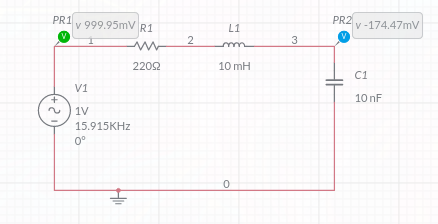
\includegraphics[width=0.6\textwidth]{../img/RLC_salida_R_circuito.png}
	\caption{Representación del circuito RLC con salida en C simulado en MultisimLive}
	\label{fig:img-RLC_salida_L-png}
\end{figure}
Para ver el valor de la tensión de salida en Multisim, simulamos el circuito para la gráfica 'Interactive', el resultado es el siguiente:
\begin{figure}[H]
	\centering
	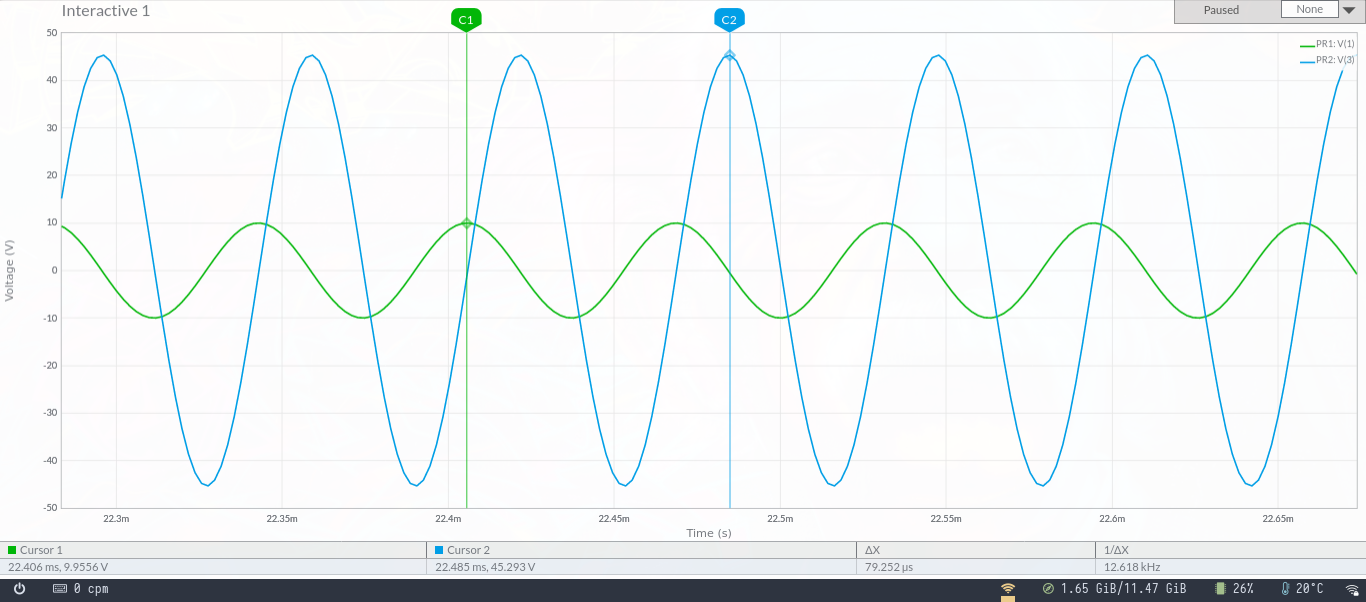
\includegraphics[width=0.8\textwidth]{../img/tension_fc_RLC_C.png}
	\caption{Representación del circuito en MultisimLive para observar la tensión de salida }
	\label{fig:}
\end{figure}
El cursor azul nos marca la tensión máxima de salida, esto es la misma que el cursor verde
\begin{figure}[H]
    \centering
    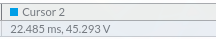
\includegraphics[width=0.4\textwidth]{../img/VmaxRLCR.png}
\end{figure}
\begin{equation}
	\boxed{V_s \approx  45.3 V}
\end{equation}
Resultado parecido al valor teórico hallado para la frecuencia de corte. 
\subsection{Comprobación experimental en el simulador ángulo de desfase}
A continuación representamos el circuito en el diagrama de Bode para poder ver el desfase que hay para la frecuencia de corte $f_n=15915.494 Hz$. Esto lo hacemos con la función AC Sweep que tiene MultisimLive:
\begin{figure}[H]
	\centering
	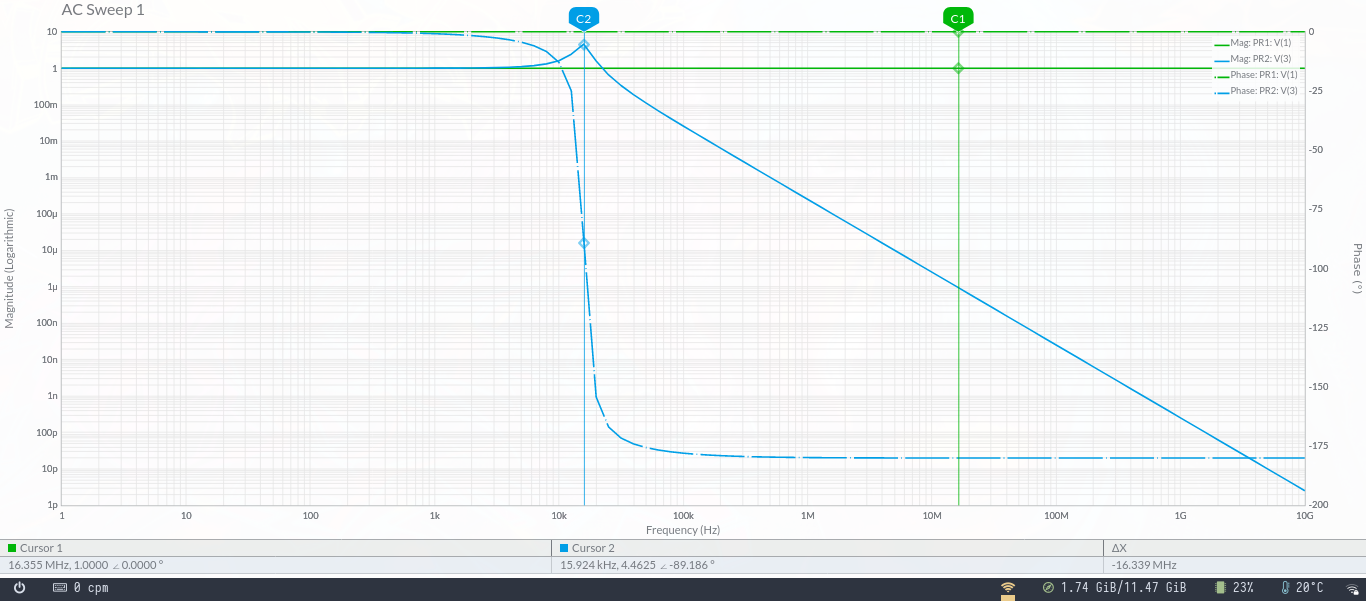
\includegraphics[width=0.8\textwidth]{../img/angulo_fc_RLC_R.png}
	\caption{Representación del diagrama de Bode del circuito para ver el desfase que se encuentra este en la frecuencia de corte}
	\label{fig:-img-angulo_fc-png}
\end{figure}
\begin{figure}[H]
    \centering
    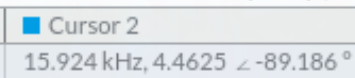
\includegraphics[width=0.4\textwidth]{../img/zoom.png}
    \label{fig:-img-zoom-png}
\end{figure}
Como vemos en la gráfica, el ángulo de desfase lo podemos encontrar cuando la función de transferencia es 4.54, esto es, para la frecuencia de corte. El ángulo de desfase corresponde con el ángulo donde ocurre el pico de la gráfica vista en la figura anterior. Aproximadamente el valor del ángulo de desfase de forma experimental es:
\begin{equation} 
	\boxed{\varphi \approx -89^o}
\end{equation}
Este valor es aproximadamente el mismo valor que hemos obtenido de forma teórica (90º). De forma que queda comprobado nuestro cálculo teórico para el ángulo de  desfase para la frecuencia de corte.
\subsection{Simulación tensión salida década por arriba}
En el diagrama de Bode podemos ver la función de transferencia para una década por arriba:
\begin{figure}[H]
    \centering
    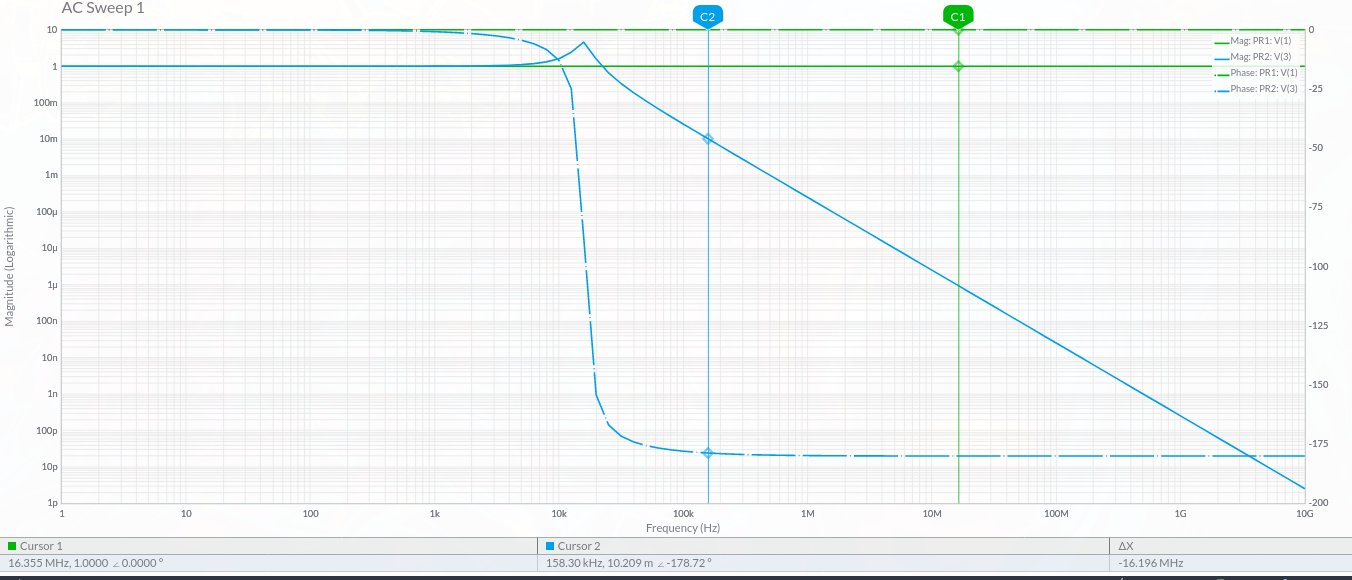
\includegraphics[width=0.8\textwidth]{../img/arriba.png}
    \label{fig:}
\end{figure}
\begin{figure}[H]
    \centering
    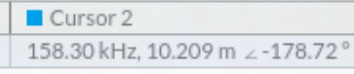
\includegraphics[width=0.4\textwidth]{../img/arriba1.png}
    \label{fig:}
\end{figure}
Como vemos, el cursor indica una década por encima de la frecuencia de corte (aproximadamente), en la que podemos ver la función de ganancia para esta frecuencia, y esta corresponde con una ganancia de 10.2. Aproximadamente el valor hallado teóricamente, haremos lo mismo una década por debajo de la frecuencia de corte.
\subsection{Simulación tensión de salida década por debajo}
Para una década por debajo, simulamos el circuito:
\begin{figure}[H]
    \centering
    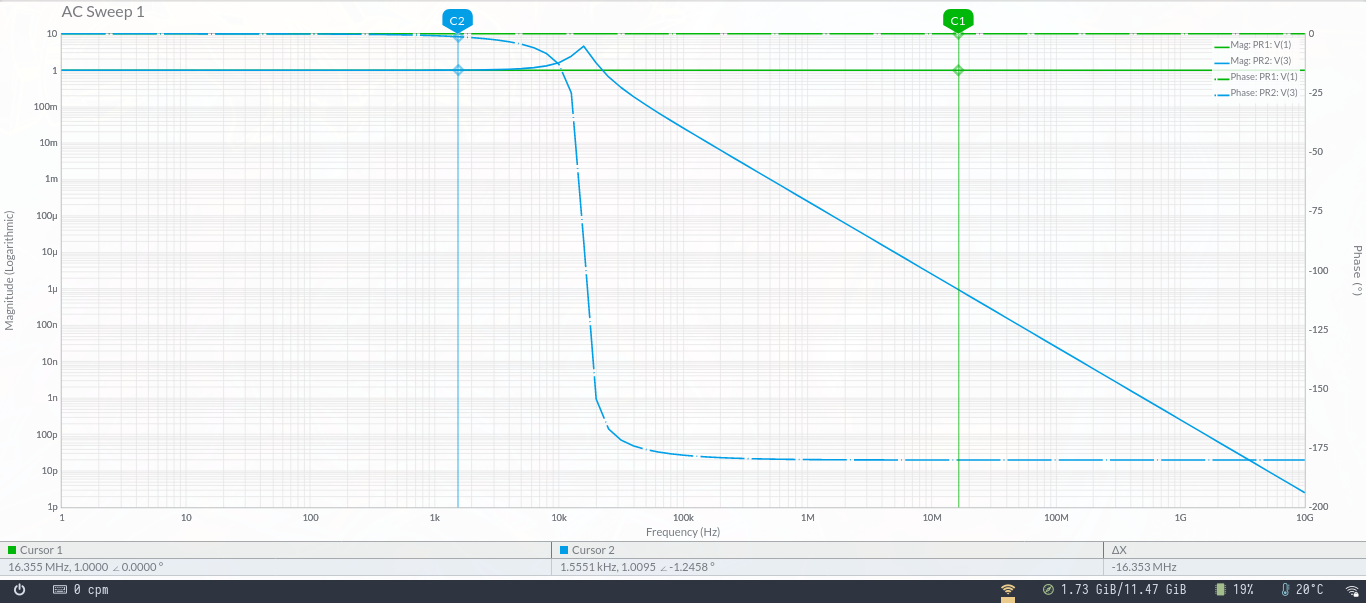
\includegraphics[width=0.8\textwidth]{../img/abajo.png}
\end{figure}    

\begin{figure}[H]
    \centering
    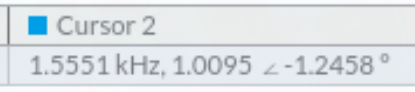
\includegraphics[width=0.4\textwidth]{../img/abajo1.png}
    \label{fig:-}
\end{figure}
Como vemos, la función de transferencia para una década por debajo es de $1$ aproximadamente. Este valor es el mismo que el hallado teóricamente. 

\subsection{Simulación tensión máxima y frecuencia máxima}
Prácticamente, es la misma que la frecuencia de corte, usamos el simulador y buscamos el pico donde el módulo de la función de transferencia es máxima, esto es:
\begin{figure}[H]
    \centering
    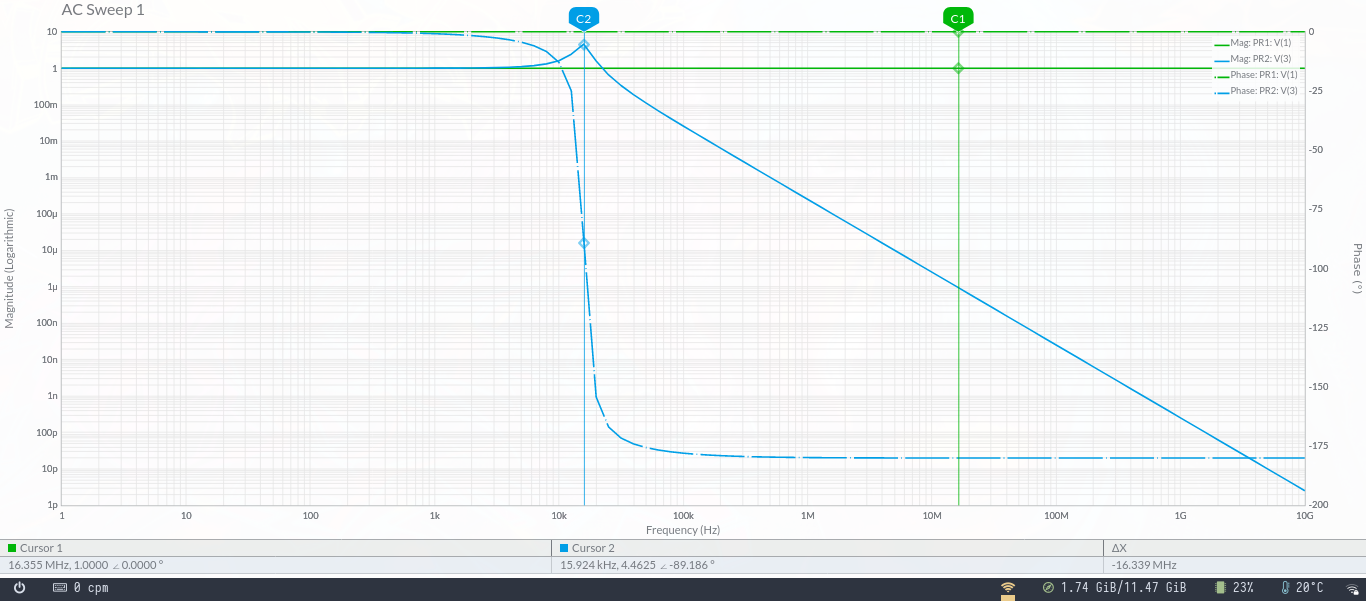
\includegraphics[width=0.8\textwidth]{../img/angulo_fc_RLC_R.png}
    \label{fig:}
\end{figure}
Donde podemos ver el valor de la función de transferencia en el pico:
\begin{figure}[H]
    \centering
    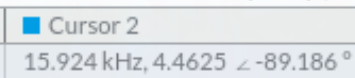
\includegraphics[width=0.4\textwidth]{../img/zoom.png}
    \label{fig:-img-zoom-png}
\end{figure}

\section{Respuesta escalón}
Representamos el circuito en el programa MultisimLive:
\begin{figure}[H]
    \centering
    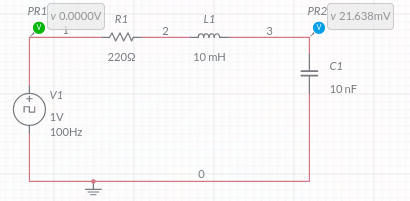
\includegraphics[width=0.8\textwidth]{../img/escalon.png}
    \caption{Represetnación del circuito con una respuesta escalón utilizando 100 Hz de frecuencia.}
    \label{fig:-img-escalon-png}
\end{figure}
La frecuencia de oscilación se calcula de forma que:
\[
w=w_n\cdot \sqrt{1-\zeta^2} 
.\] 
Sustituyendo tal que la frecuencia de corte es : $w_n=15915.494Hz$
\[
\omega= 15918.90 Hz
.\] 
Podemos ver la simulación en Multisim, de forma que entre pico y pico máximo podemos obtener el valor de la frecuencia , es decir,frecuencia para un periodo, esto es:
\begin{figure}[H]
    \centering
    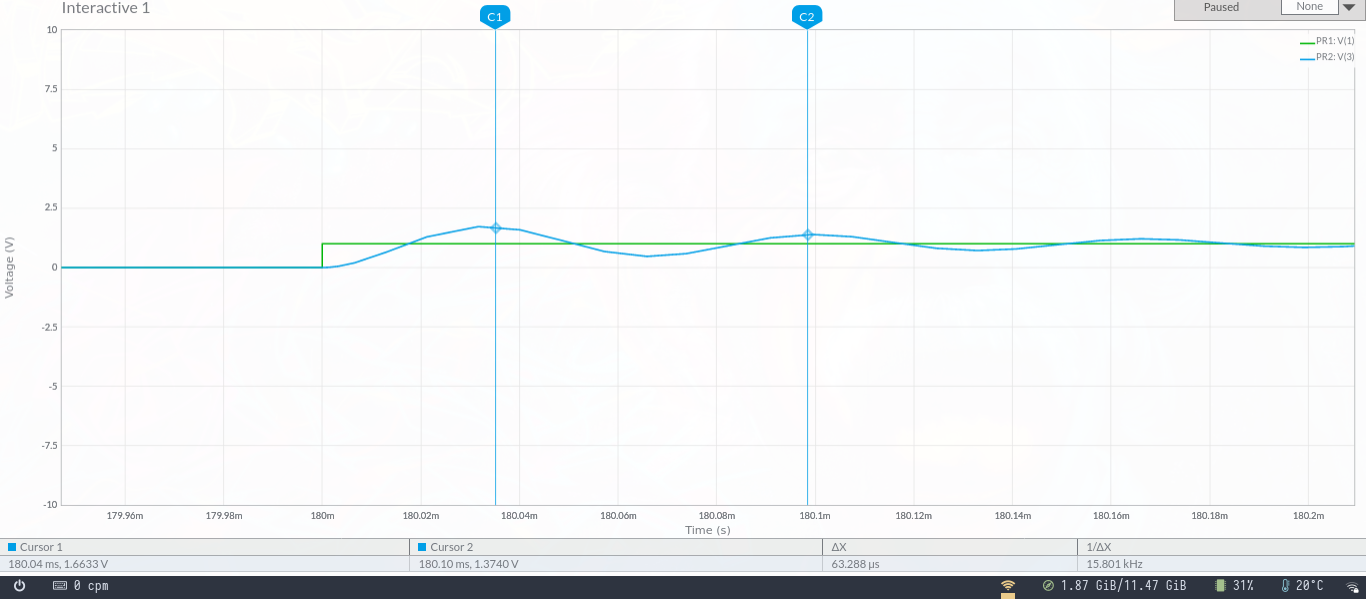
\includegraphics[width=0.8\textwidth]{../img/escalon1.png}
    \label{fig:-img-escalon1-png}
\end{figure}
\begin{figure}[H]
    \centering
    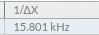
\includegraphics[width=0.4\textwidth]{../img/escalon2.png}
    \label{fig:-img-escalon2-png}
\end{figure}
 Por tanto, la frecuencia hallada en el simulador es :
 \[
 \omega \approx 15801 Hz
 .\] 
 Valor parecido al teórico anteriormente calculado.

 \section{Conclusiones del comportamiento de este circuito}
 El comportamiento de este circtuito se puede ver con los cálculos de la función de transferencia para frecuencias altas y bajas. Como hemos visto, cuando la frecuencia está por encima de la frecuencia de corte, la función de ganancia disminuye y al contrario, cuando la frecuencia está por debajo de la frecuencia de corte, la función de ganancia aumenta. Esto quiere decir que el circuito está filtrando las frecuencias bajas, atenunando las frecuencias altas. Esto es, es un circuito de paso bajo. 
$\mathbf{W} $
 \end{document}
